\documentclass[12pt]{article}
\usepackage{amsthm,amssymb,amsmath,amsfonts}
\usepackage[a4paper, top=25mm, bottom=30mm, left=25mm, right=25mm]{geometry}
\usepackage[pagebackref=false,colorlinks,linkcolor=black,citecolor=black]{hyperref}
\usepackage[nameinlink]{cleveref}
 \AtBeginDocument{%
    \crefname{equation}{برابری}{equations}%
    \crefname{chapter}{فصل}{chapters}%
    \crefname{section}{بخش}{sections}%
    \crefname{appendix}{پیوست}{appendices}%
    \crefname{enumi}{مورد}{items}%
    \crefname{footnote}{زیرنویس}{footnotes}%
    \crefname{figure}{شکل}{figures}%
    \crefname{table}{جدول}{tables}%
    \crefname{theorem}{قضیه}{theorems}%
    \crefname{lemma}{لم}{lemmas}%
    \crefname{corollary}{نتیجه}{corollaries}%
    \crefname{proposition}{گزاره}{propositions}%
    \crefname{definition}{تعریف}{definitions}%
    \crefname{result}{نتیجه}{results}%
    \crefname{example}{مثال}{examples}%
    \crefname{remark}{نکته}{remarks}%
    \crefname{note}{یادداشت}{notes}%
    \crefname{observation}{مشاهده}{observations}%
    \crefname{algorithm}{الگوریتم}{algorithms}%
    \crefname{cproof}{برهان}{cproofs}%
}

\usepackage{tikz}
\usepackage{graphicx}
\usepackage{booktabs}
\usepackage{color}
\usepackage{graphicx}
\usepackage{subcaption}

\usepackage{setspace}
\doublespacing

\usepackage{titletoc}
\usepackage{tocloft}
\usepackage{enumitem}
\usepackage{amsmath, amssymb}
\usepackage{algorithm}
\usepackage[noend]{algorithmic}
\renewcommand{\algorithmicrequire}{\textbf{Input:}}
\renewcommand{\algorithmicensure}{\textbf{Output:}}

\usepackage{tabularx}
\makeatletter
\newcommand{\multiline}[1]{%
  \begin{tabularx}{\dimexpr\linewidth-\ALG@thistlm}[t]{@{}X@{}}
    #1
  \end{tabularx}
}
\makeatother

\usepackage{float}
\usepackage{verbatim}
\makeindex
\usepackage{sectsty}
\usepackage{xepersian}
\SepMark{-}
\settextfont[Scale=1.2,Path=fonts/,BoldFont=B Nazanin Bold.ttf]{B Nazanin.ttf}
\setlatintextfont{Times New Roman}
\renewcommand{\labelitemi}{$\bullet$}

\theoremstyle{definition}
\newtheorem{definition}{تعریف}[section]
\newtheorem{remark}[definition]{نکته}
\newtheorem{note}[definition]{یادداشت}
\newtheorem{example}[definition]{نمونه}
\newtheorem{question}[definition]{سوال}
\newtheorem{remember}[definition]{یاداوری}
\newtheorem{observation}[definition]{مشاهده}
\theoremstyle{theorem}
\newtheorem{theorem}[definition]{قضیه}
\newtheorem{lemma}[definition]{لم}
\newtheorem{proposition}[definition]{گزاره}
\newtheorem{corollary}[definition]{نتیجه}
\newtheorem*{cproof}{برهان}




\begin{document}
\fontsize{12pt}{14pt}\selectfont

\begin{minipage}{0.1\textwidth}

\includegraphics[width=3cm]{etc/IUST}
\end{minipage}%
\hfill%
\begin{minipage}{0.6\textwidth}\centering
\fontsize{13pt}{13pt}\selectfont
به‌ نام خدا \\
\textbf{درس یادگیری عمیق} \\
\textbf{تمرین سری ششم}\\
استاد درس : دکتر محمدرضا محمدی \\
دستیاران :  مهدی خورشا، سید محمد موسوی،\\ امیرحسین نمازی
\\
\vspace{0.25cm}
\begingroup
\fontsize{11pt}{11pt}\selectfont
دانشگاه علم و صنعت ایران، دانشکده مهندسی کامپیوتر \\
نیمسال دوم تحصیلی 1403 - 1404 \\
\endgroup
\end{minipage}%
\hfill%
\begin{minipage}{0.1\textwidth}

\end{minipage}

\vspace{0.5cm}

\noindent\rule{\textwidth}{1pt}

\centering {\fontsize{18}{22}\selectfont \textbf{مهلت تحویل : 1404/02/23 }}\\
{\fontsize{14}{22}\selectfont \textbf{لطفا به نکات موجود در سند قوانین انجام و تحویل تمرین ها دقت فرمایید. }}

\begin{enumerate}

    \section*{سوالات تئوری}
    \item 
\includegraphics[width=1cm]{figs/Forbidden_AI.jpg}
    بر اساس \href{https://arxiv.org/abs/2309.06180}{ مقاله} لطفا به سوالات زیر پاسخ دهید (۱۰ نمره):
    \begin{enumerate}
        \item چالش‌های اصلی در زمینه مدیریت حافظه که سیستم‌های خدمات‌دهی \lr{LLM} موجود مواجه هستند، چیست؟
        
        \textcolor{blue}{
        سیستم‌های خدمات‌دهی \lr{LLM} موجود به دلیل نحوه مدیریت حافظه کش کلید-مقدار \LTRfootnote{KV Cache} با چالش‌های اساسی مواجه هستند. مشکل اصلی این است که این سیستم‌ها حافظه کش \lr{KV} هر درخواست را در یک فضای حافظه پیوسته\LTRfootnote{contiguous} ذخیره می‌کنند. این رویکرد به دلیل ویژگی‌های منحصربه‌فرد حافظه کش \lr{KV} در \lr{LLM}ها (رشد پویا، طول عمر و اندازه نامشخص از قبل) منجر به ناکارآمدی‌های جدی می‌شود.
        چالش‌های اصلی عبارتند از:
        \begin{enumerate}
            \item اتلاف حافظه به دلیل تکه‌تکه شدن\LTRfootnote{Fragmentation}:
            \begin{itemize}
                \item تکه‌تکه شدن داخلی\LTRfootnote{Internal Fragmentation} : سیستم‌های موجود برای هر درخواست، یک قطعه حافظه پیوسته به اندازه حداکثر طول دنباله ممکن (مثلاً ۲۰۴۸ توکن) از پیش تخصیص می‌دهند. از آنجایی که طول واقعی خروجی اغلب بسیار کوتاه‌تر از این مقدار است، بخش بزرگی از حافظه تخصیص‌داده‌شده هرگز استفاده نمی‌شود و به هدر می‌رود. (ارجاع: بخش ۱ و شکل ۳). مقاله در شکل ۲ نشان می‌دهد که در سیستم‌های موجود، تنها ۲۰ تا ۳۸ درصد از حافظه کش \lr{KV} واقعاً برای ذخیره توکن‌ها استفاده می‌شود.
                \item تکه‌تکه شدن خارجی\LTRfootnote{External Fragmentation}: زمانی که درخواست‌ها با طول‌های حداکثری متفاوت وارد سیستم می‌شوند، تخصیص‌دهنده حافظه (مانند \lr{buddy allocator}) ممکن است نتواند فضاهای خالی بین بلاک‌های تخصیص‌داده‌شده را به طور مؤثر مدیریت کند و فضاهای خالی غیرقابل استفاده‌ای ایجاد می‌شود. (ارجاع: بخش ۱ و شکل ۳).
                تصور کنید حافظه \lr{GPU} شما یک قفسه کتاب با طول مشخص است. هر درخواست\LTRfootnote{request} یک کتاب با قطر متفاوت است.
                \begin{figure}[h]
                    \centering
                    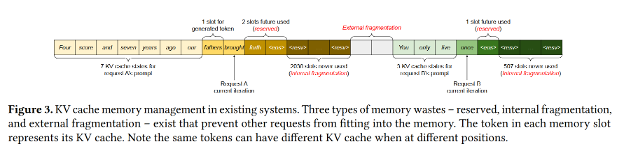
\includegraphics[width=\textwidth]{figs/Q1_1.png}
                    \label{fig:num_pic}  
                \end{figure}
                حالت سیستم‌های قدیمی (تکه‌تکه شدن خارجی): این سیستم‌ها برای هر کتاب (درخواست) نیاز به یک فضای یکپارچه و پیوسته روی قفسه دارند. فرض کنید یک کتاب با قطر ۲۰ سانتی‌متر و یک کتاب با قطر ۳۰ سانتی‌متر را در قفسه قرار می‌دهید. حالا یک کتاب با قطر ۵۰ سانتی‌متر برداشته می‌شود. اکنون شما یک فضای خالی ۵۰ سانتی‌متری دارید. اگر درخواست بعدی یک کتاب با قطر ۶۰ سانتی‌متر باشد، با اینکه مجموع فضاهای خالی در کل قفسه شاید بیشتر از ۶۰ سانتی‌متر باشد، اما چون هیچ فضای خالی یکپارچه‌ای به طول ۶۰ سانتی‌متر وجود ندارد، این کتاب جدید در قفسه جا نمی‌شود. این فضاهای خالیِ کوچک و پراکنده که قابل استفاده برای درخواست‌های بزرگتر نیستند، تکه‌تکه شدن خارجی نام دارند. مقاله در شکل ۳ به خوبی این مفهوم را نشان می‌دهد که فضاهای خالی بین بلاک‌های حافظه‌ی رزرو شده برای درخواست \lr{A} و \lr{B} وجود دارد که قابل استفاده نیستند.
            \end{itemize}
            \item عدم امکان اشتراک‌گذاری حافظه\LTRfootnote{Inability to Share Memory}:	الگوریتم‌های رمزگشایی پیشرفته مانند نمونه‌برداری موازی\LTRfootnote{Parallel Sampling} یا جستجوی پرتوئی\LTRfootnote{Beam Search} چندین دنباله خروجی برای یک ورودی واحد تولید می‌کنند. بخش‌هایی از این دنباله‌ها (مانند پرامپت اولیه) کاملاً یکسان هستند و حافظه کش \lr{KV} آن‌ها می‌تواند به اشتراک گذاشته شود. اما چون سیستم‌های موجود برای هر دنباله یک بلاک حافظه پیوسته مجزا تخصیص می‌دهند، این اشتراک‌گذاری حافظه غیرممکن یا بسیار ناکارآمد است. (ارجاع: بخش ۱ و بخش ۳، پاراگراف \lr{Complex decoding algorithms}).
            \item حافظه کش \lr{KV} و محدودیت‌های برنامه‌ریزی\LTRfootnote{Large KV Cache \& Scheduling Complexity}:
            \begin{itemize}
                \item حافظه کش \lr{KV} برای هر درخواست می‌تواند بسیار بزرگ باشد (مثلاً تا \lr{۱.۶} گیگابایت برای یک درخواست در مدل \lr{OPT-13B}). این امر تعداد درخواست‌هایی را که می‌توانند به صورت همزمان در یک دسته \LTRfootnote{batch} پردازش شوند، به شدت محدود می‌کند. (ارجاع: بخش ۳، پاراگراف \lr{Large KV cache}).
                \item طول ورودی و خروجی درخواست‌ها از قبل مشخص نیست. این عدم قطعیت، برنامه‌ریزی\LTRfootnote{scheduling} و تخصیص حافظه را پیچیده می‌کند و باعث می‌شود سیستم‌ها رویکرد محافظه‌کارانه و ناکارآمد تخصیص حداکثری را در پیش بگیرند. (ارجاع: بخش ۳، پاراگراف \lr{Scheduling for unknown input/output lengths}).
            \end{itemize}
        \end{enumerate}}
        
        \item  \lr{PagedAttention} چگونه به این چالش‌ها پاسخ می‌دهد؟ 
        
        \textcolor{blue}{
        \lr{PagedAttention} یک الگوریتم توجه\LTRfootnote{Attention} جدید است که با الهام از تکنیک‌های کلاسیک حافظه مجازی\LTRfootnote{Virtual Memory} و صفحه‌بندی\LTRfootnote{Paging} در سیستم‌عامل‌ها طراحی شده است تا مشکلات مدیریت حافظه در سیستم‌های موجود را حل کند.
        \begin{figure}[h]
            \centering
            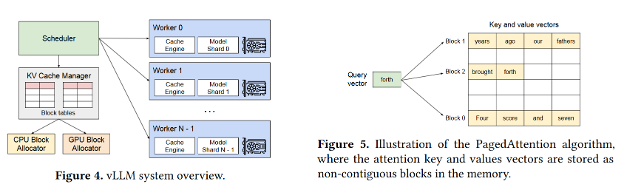
\includegraphics[width=\textwidth]{figs/Q1_2.png}
            \label{fig:num_pic}  
        \end{figure}
        \begin{figure}[h]
            \centering
            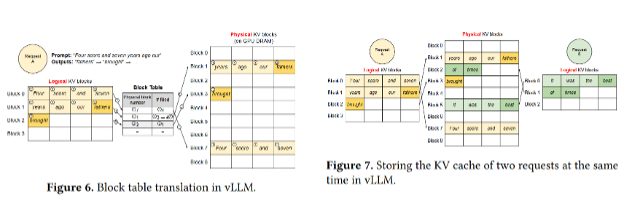
\includegraphics[width=\textwidth]{figs/Q1_21.png}
            \label{fig:num_pic}  
        \end{figure}
        راهکار اصلی \lr{PagedAttention} این است که به کلیدها و مقادیر (\lr{KV Cache}) اجازه می‌دهد تا در فضاهای حافظه غیرپیوسته\LTRfootnote{non-contiguous} ذخیره شوند. این کار از طریق مکانیزم زیر انجام می‌شود:
        \begin{enumerate}
            \item تقسیم حافظه کش به بلاک‌ها (\lr{KV Blocks}): \lr{PagedAttention} حافظه کش \lr{KV} هر دنباله را به بلاک‌هایی با اندازه ثابت تقسیم می‌کند. هر بلاک، کلید و مقدار مربوط به تعداد ثابتی از توکن‌ها را در خود جای می‌دهد. این بلاک‌ها معادل “صفحات\LTRfootnote{Pages}”  در حافظه مجازی هستند. (ارجاع: بخش \lr{۴.۱}).
            \item مدیریت غیرپیوسته حافظه: برخلاف سیستم‌های قبلی، این بلاک‌ها نیازی به قرارگیری پشت سر هم در حافظه فیزیکی \lr{GPU} ندارند. \lr{vLLM} با استفاده از جداول بلاک\LTRfootnote{Block Tables}، بلاک‌های منطقی (از دید هر دنباله) را به بلاک‌های فیزیکی (در حافظه \lr{GPU}) نگاشت می‌کند. (ارجاع: بخش \lr{۴.۲} و شکل ۵ و ۶).
        \end{enumerate}
        \lr{PagedAttention} با این رویکرد به چالش‌های ذکر شده در سوال (آ) به شکل زیر پاسخ می‌دهد:
        \begin{itemize}
            \item حل مشکل تکه‌تکه شدن:
            \begin{itemize}
                \item تکه‌تکه شدن داخلی: حافظه به صورت پویا و بلاک به بلاک تخصیص داده می‌شود. یعنی تنها زمانی یک بلاک جدید تخصیص می‌یابد که بلاک قبلی پر شده باشد. این کار اتلاف حافظه داخلی را به حداکثر یک بلاک برای هر دنباله محدود می‌کند که بسیار ناچیز است. (ارجاع: بخش \lr{۴.۳}).
                \item تکه‌تکه شدن خارجی: از آنجایی که تمام بلاک‌ها اندازه یکسانی دارند، مشکل تکه‌تکه شدن خارجی به طور کامل از بین می‌رود. (ارجاع: بخش ۱).
            \end{itemize}
            \item امکان‌پذیر کردن اشتراک‌گذاری حافظه: از آنجا که هر بلاک به صورت مستقل مدیریت می‌شود، چندین دنباله منطقی می‌توانند به یک بلاک فیزیکی واحد اشاره کنند. این قابلیت، اشتراک‌گذاری حافظه را به سادگی ممکن می‌سازد. (ارجاع: بخش \lr{۴.۴}).
        \end{itemize}
        در نتیجه، \lr{PagedAttention} با حذف اتلاف حافظه، به سیستم اجازه می‌دهد تا درخواست‌های بیشتری را در یک بچ قرار دهد و توان عملیاتی\LTRfootnote{throughput} را به شدت افزایش دهد. (ارجاع: شکل ۲ که نشان می‌دهد \lr{vLLM} نزدیک به صفر اتلاف حافظه دارد).
        }
        
        \item اهمیت اشتراک‌گذاری حافظه کش \lr{KV} در سیستم‌های خدمات‌دهی \lr{LLM} را مورد بحث قرار دهید. \lr{vLLM} چگونه اشتراک‌گذاری حافظه را تسهیل می‌کند و این موضوع چه پیامدهایی برای توان عملیاتی کلی سیستم دارد؟ پاسخ خود را با جزئیات موجود در مقاله بیان کنید.
        
        \textcolor{blue}{
        \begin{enumerate}
            \item اهمیت اشتراک‌گذاری حافظه کش \lr{KV}: اشتراک‌گذاری حافظه کش \lr{KV} در سناریوهای رایج سرویس‌دهی \lr{LLM} بسیار حیاتی است، زیرا مستقیماً منجر به صرفه‌جویی در مصرف حافظه می‌شود. سناریوهای کلیدی عبارتند از:
            \begin{figure}[h]
                \centering
                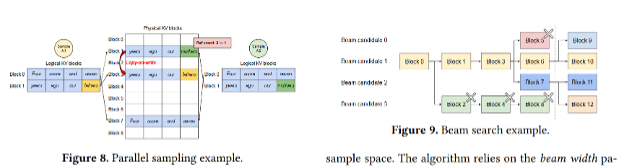
\includegraphics[width=\textwidth]{figs/Q1_3.png}
                \label{fig:num_pic}  
            \end{figure}
            \begin{itemize}
                \item نمونه‌برداری موازی\LTRfootnote{Parallel Sampling}: زمانی که برای یک پرامپت ورودی، چندین خروجی مستقل تولید می‌شود (مثلاً برای ارائه گزینه‌های مختلف به کاربر). در این حالت، حافظه کش \lr{KV} مربوط به پرامپت اولیه بین تمام خروجی‌ها مشترک است. (ارجاع: بخش \lr{۴.۴}).
                \item جستجوی پرتوئی\LTRfootnote{Beam Search}: در این الگوریتم، چندین “کاندیدا” برای بهترین خروجی به صورت همزمان بررسی می‌شوند. این کاندیداها نه تنها در پرامپت، بلکه در بخش‌های ابتدایی توالی تولید شده نیز اشتراک دارند. الگوی اشتراک به صورت پویا در هر مرحله تغییر می‌کند. (ارجاع: بخش \lr{۴.۴} و شکل ۹).
                \item پیشوند مشترک\LTRfootnote{Shared Prefix}: در بسیاری از کاربردها، یک پیشوند طولانی (مانند دستورالعمل‌ها یا مثال‌ها) به تمام درخواست‌ها اضافه می‌شود. با ذخیره کردن حافظه کش \lr{KV} این پیشوند، می‌توان از محاسبات تکراری جلوگیری کرد. (ارجاع: بخش \lr{۴.۴} و شکل ۱۰).
            \end{itemize}
            \item نحوه تسهیل اشتراک‌گذاری حافظه در \lr{vLLM}: \lr{vLLM} با استفاده از مکانیزم‌های الهام‌گرفته از سیستم‌عامل، اشتراک‌گذاری حافظه را به طور کارآمد پیاده‌سازی می‌کند:
            \begin{itemize}
                \item جداول بلاک و نگاشت چند به یک: \lr{vLLM} به هر دنباله یک جدول بلاک منطقی اختصاص می‌دهد. این سیستم اجازه می‌دهد که چندین بلاک منطقی از دنباله‌های مختلف به یک بلاک فیزیکی واحد در حافظه \lr{GPU} نگاشت شوند. (ارجاع: بخش \lr{۴.۲} و \lr{۴.۴}).
                \item شمارش ارجاع\LTRfootnote{Reference Counting}: برای هر بلاک فیزیکی یک شمارنده ارجاع نگهداری می‌شود. این شمارنده تعداد دنباله‌های منطقی را که به آن بلاک اشاره می‌کنند، ثبت می‌کند. یک بلاک فیزیکی تنها زمانی آزاد می‌شود که شمارنده ارجاع آن به صفر برسد. (ارجاع: بخش \lr{۴.۴}، زیربخش \lr{Parallel sampling}).
                \item کپی در زمان نوشتن\LTRfootnote{Copy-on-Write - CoW}: زمانی که یک دنباله نیاز به تغییر محتوای یک بلاک مشترک دارد (مثلاً با اضافه کردن یک توکن جدید)، \LTRfootnote{vLLM} به جای تغییر بلاک اصلی، یک کپی جدید از آن بلاک ایجاد می‌کند، آن را به دنباله مورد نظر اختصاص می‌دهد و شمارنده ارجاع بلاک اصلی را کاهش می‌دهد. این کار از کپی‌های غیرضروری جلوگیری کرده و تنها در مواقع لزوم انجام می‌شود. (ارجاع: بخش \lr{۴.۴} و شکل ۸).
            \end{itemize}
            \item پیامدها برای توان عملیاتی\LTRfootnote{Throughput}: اشتراک‌گذاری حافظه به طور مستقیم توان عملیاتی کل سیستم را افزایش می‌دهد. این تأثیر به شکل زیر است:
            \begin{itemize}
                \item کاهش مصرف حافظه: با اشتراک‌گذاری، حافظه مورد نیاز برای هر گروه از درخواست‌ها (مثلاً یک درخواست با چندین خروجی موازی) به شدت کاهش می‌یابد. مقاله در شکل ۱۵ نشان می‌دهد که این روش می‌تواند در \lr{Parallel Sampling} تا \lr{۳۰٪} و در \lr{Beam Search} تا \lr{۶۶٪} حافظه را صرفه‌جویی کند.
                \item افزایش اندازه بچ\LTRfootnote{Batch Size}: صرفه‌جویی در حافظه به \lr{vLLM} اجازه می‌دهد تا تعداد بسیار بیشتری درخواست را به صورت همزمان در یک بچ قرار دهد. (ارجاع: شکل ۱۳ که افزایش چشمگیر تعداد درخواست‌های بچ‌شده را نشان می‌دهد).
                \item افزایش توان عملیاتی: افزایش اندازه بچ به معنای استفاده بهینه‌تر از قدرت محاسباتی \lr{GPU} و در نتیجه، افزایش قابل توجه توان عملیاتی (تعداد درخواست‌های پردازش شده در ثانیه) است. مقاله در بخش \lr{۶.۳} و شکل ۱۴ نشان می‌دهد که مزیت توان عملیاتی \lr{vLLM} نسبت به سیستم‌های دیگر در سناریوهای \lr{Beam Search} (که اشتراک‌گذاری بیشتری دارند) بسیار بارزتر است. برای مثال، برتری \lr{vLLM} نسبت به \lr{Orca} از \lr{۱.۳} برابر در نمونه‌برداری عادی به \lr{۲.۳} برابر در \lr{Beam Search} با عرض ۶ افزایش می‌یابد.
            \end{itemize}
        \end{enumerate}}
    \end{enumerate}
    
    \href{https://www.youtube.com/watch?v=5ZlavKF_98U}{ویدیوی ارائه نویسندگان مقاله در یک کنفرانس}

    \item 
\includegraphics[width=1cm]{figs/Forbidden_AI.jpg}
    	با توجه به \lr{Multi-Head Attention} به پرسش‌های زیر پاسخ دهید (10 نمره):
        \begin{enumerate}
            \item	چرا در مدل‌های ترنسفورمر از توجه چندسری (\lr{Multi-Head Attention}) استفاده می‌شود؟ و این سرهای توجه چه نوع اطلاعاتی را می‌توانند یاد بگیرند؟
            
            \textcolor{blue}{
                مدل‌های ترنسفورمر برای یادگیری بهتر و دقیق‌تر از توجه چندسری استفاده می‌کنند. دلایل اصلی آن عبارتند از:
                \begin{itemize}
                    \item نمایش‌های متنوع\LTRfootnote{Diverse Representations}:
                    هر سر توجه می‌تواند بر بخش متفاوتی از دنباله ورودی تمرکز کند و روابط و الگوهای مختلفی را بیاموزد. این تنوع در توجه، باعث افزایش قدرت مدل در درک داده‌های پیچیده می‌شود.
                    \item افزایش ظرفیت مدل\LTRfootnote{Increased Capacity}:
                    با داشتن چندین سر توجه، مدل می‌تواند اطلاعات بیشتری را به‌صورت همزمان پردازش کند. هر سر می‌تواند در ویژگی خاصی تخصص پیدا کند و در نتیجه، نمایش نهایی غنی‌تری حاصل شود.
                    \item پویایی بهتر در یادگیری\LTRfootnote{Improved Learning Dynamics}:
                    یادگیری جنبه‌های مختلف داده توسط سرهای مختلف، به مدل کمک می‌کند تا از بیش‌برازش\LTRfootnote{Overfitting} جلوگیری کرده و عملکرد بهتری روی داده‌های نادیده از خود نشان دهد.
                    \item درک بهتر زمینه\LTRfootnote{Enhanced Contextual Understanding}:
                    هر سر توجه می‌تواند به زمینه یا جنبه متفاوتی از ورودی توجه کند، که موجب درک بهتر مفاهیم و ظرایف زبانی یا سایر داده‌های ترتیبی می‌شود.
                    \item پردازش تانسوری و موازی\LTRfootnote{Tensor Processing \& Parallelism}:
                    محاسبات مستقل هر سر توجه امکان استفاده از عملیات تانسوری و اجرای موازی را فراهم می‌سازد که موجب افزایش سرعت آموزش و پیش‌بینی می‌شود.
                    \item الگوهای توجه انعطاف‌پذیر\LTRfootnote{Flexibility in Attention Patterns}:
                    سرهای مختلف می‌توانند به انواع مختلفی از وابستگی‌ها در داده‌ها (مثل وابستگی‌های محلی و سراسری) توجه کنند و این امر موجب افزایش تطبیق‌پذیری مدل در مواجهه با مسائل مختلف می‌شود.
                \end{itemize}}
            
            \item 	فرض کنید یک مدل آموزش‌دیده داریم که بر پایه‌ی توجه چندسری (\lr{Multi-Head Attention}) ساخته شده است و می‌خواهیم برای افزایش سرعت پیش‌بینی، سرهای توجه کم‌اهمیت‌تر را حذف (\lr{Prune}) کنیم. چگونه می‌توانیم آزمایش‌هایی طراحی کنیم تا اهمیت هر سر توجه را اندازه‌گیری کنیم؟
            
            \textcolor{blue}{
            برخی از روش‌ها عبارتند از:
            \begin{itemize}
                \item آزمون حذف تدریجی\LTRfootnote{Ablation Study}:
                در این روش، هر سر توجه به‌صورت جداگانه غیرفعال می‌شود (خروجی‌اش صفر یا حذف می‌شود) و عملکرد مدل روی داده‌های اعتبارسنجی\LTRfootnote{Validation} اندازه‌گیری می‌شود.
                مراحل:
                \begin{itemize}
                    \item یکی از \lr{Head} ها را حذف کن.
                    \item مدل را اجرا کن و دقت یا معیار ارزیابی (\lr{Accuracy}, \lr{BLEU}, \lr{F1} و ...) را ثبت کن.
                    \item همین کار را برای تک‌تک \lr{Head} ها تکرار کن.
                    \item کاهش زیاد در عملکرد = اهمیت بالا و کاهش کم یا بدون تأثیر = اهمیت پایین
                \end{itemize}
                \item تحلیل بر اساس گرادیان‌ها\LTRfootnote{Gradient-based Analysis}:
                در این روش، اندازه گرادیان‌های مربوط به وزن‌های هر \lr{Head} بررسی می‌شود. گرادیان‌های کم نشان می‌دهند که \lr{head} در طول آموزش به‌روزرسانی خاصی دریافت نکرده و احتمالاً کم‌اهمیت است. مراحل:
                \begin{itemize}
                    \item در طول آموزش یا \lr{inference}، گرادیان وزن‌های ماتریس‌های  \lr{Q، K،V}  برای هر  \lr{Head} را ذخیره کن.
                    \item میانگین یا نُرم \lr{L2} این گرادیان‌ها را محاسبه کن.
                    \item \lr{Head} هایی با گرادیان کوچک \lr{→} احتمالاً  بلااستفاده یا کم‌اهمیت هستند.
                \end{itemize}
                \item آنتروپی توجه\LTRfootnote{Attention Entropy}:
                سرهایی که توجه یکنواخت و پخش دارند (توجه به همه توکن‌ها به یک میزان)، اطلاعات خاصی منتقل نمی‌کنند. می‌توان با محاسبه آنتروپی \lr{distribution} توجه، به این موضوع پی برد.
                مراحل:
                \begin{itemize}
                    \item ماتریس \lr{attention weights} هر \lr{Head} را بگیر.
                    \item برای هر سطر (\lr{query})، آنتروپی آن را محاسبه کن.
                    \item آنتروپی بالا = توجه پخش \lr{Head} \lr{→} کم‌اهمیت
                    \item آنتروپی پایین = توجه متمرکز \lr{Head} \lr{→} مهم‌تر
                \end{itemize}
            \end{itemize}
            }
            \item 	حذف سرهای توجه چه اثری روی وظایف پایین‌دستی (مثل طبقه‌بندی یا ترجمه) دارد؟ از چه معیارهایی برای ارزیابی تأثیر حذف سرها استفاده کنیم؟
            \textcolor{blue}{
            \begin{itemize}
                \item کاهش دقت مدل\lr{Performance Degradation}:
                اگر \lr{head} هایی حذف شوند که اطلاعات مهمی از ورودی را منتقل می‌کردند، ممکن است دقت مدل کاهش یابد، مخصوصاً در وظایف حساس به زمینه\LTRfootnote{context-sensitive tasks} مانند ترجمه.
                \item افزایش سرعت پیش‌بینی\LTRfootnote{Faster Inference}:
                با کاهش تعداد \lr{head} ها، محاسبات \lr{matrix-multiplication} برای  \lr{Q،K} و \lr{V} کاهش یافته و سرعت \lr{inference} بیشتر می‌شود.
                \item کاهش مصرف حافظه\LTRfootnote{Memory \& Resource Efficiency}:
                حذف \lr{head} ها باعث می‌شود حافظه \lr{GPU/CPU} کمتر مصرف شود، خصوصاً در مدل‌های بزرگ مانند \lr{BERT} یا \lr{GPT}.
                \item احتمال بهبود تعمیم‌پذیری\LTRfootnote{Generalization}:
                در برخی موارد، حذف \lr{head} های غیرمفید می‌تواند باعث  کاهش بیش‌برازش و بهبود تعمیم‌پذیری مدل روی داده‌های جدید شود.
                \item ریسک حذف اطلاعات حیاتی:
                اگر فرآیند \lr{pruning} به‌درستی انجام نشود، ممکن است \lr{head} های مهم حذف شوند و این منجر به افت شدید   عملکرد شود.
            \end{itemize}
            برای ارزیابی اینکه حذف سرهای توجه چه تأثیری داشته، می‌توان از معیارهای زیر استفاده کرد:
            \begin{itemize}
                \item معیارهای عملکرد مدل:
                \begin{itemize}
                    \item در طبقه‌بندی:
                    \begin{itemize}
                        \item \lr{Accuracy}
                        \item \lr{F1 Score}
                        \item \lr{Precision / Recall}
                    \end{itemize}
                    \item در ترجمه ماشینی:
                    \begin{itemize}
                        \item \lr{BLEU Score}
                        \item \lr{METEOR / ROUGE}
                    \end{itemize}
                \end{itemize}
                \item معیارهای منابع محاسباتی:
                \begin{itemize}
                    \item زمان پیش‌بینی:
                    مقایسه زمان پردازش یک نمونه بین مدل \lr{pruning‌شده}  و مدل اصلی.
                    \item تعداد پارامترها:
                    بررسی میزان کاهش پارامترهای مدل پس از حذف \lr{head} ها.
                    \item تعداد عملیات شناور\LTRfootnote{FLOPs}:
                    مقایسه حجم محاسبات قبل و بعد از  \lr{pruning}.
                    \item میزان استفاده از حافظه:
                    در مدل‌های بزرگ، حذف \lr{head} ها می‌تواند مصرف حافظه  را کاهش دهد.
                \end{itemize}
                \item معیارهای تحلیلی و ساختاری
                \begin{itemize}
                    \item تحلیل آنتروپی توجه\LTRfootnote{Attention Entropy}:
                    بررسی تغییرات در الگوهای توجه پس از حذف \lr{head} ها.
                    \item تغییر در بردارهای ویژگی\LTRfootnote{Embedding Drift}:
                    تحلیل اینکه حذف \lr{head} ها چه اثری بر نمایش نهایی داده‌ها می‌گذارد.
                \end{itemize}
            \end{itemize}
            }
            \item آیا می‌توان از یادگیری تقویتی \LTRfootnote{Reinforcement Learning} برای انتخاب دینامیک سرهای توجه استفاده کرد؟
            
            \textcolor{blue}{
            بله، می‌توان از یادگیری تقویتی برای انتخاب دینامیک (پویا) سرهای توجه در مدل‌های ترنسفورمر استفاده کرد. این ایده در برخی پژوهش‌ها و مقالات نیز پیاده‌سازی شده و به نتایج جالبی منجر شده است.
            }
        \end{enumerate}
        (اختیاری: می‌توانید از \href{https://arxiv.org/abs/1905.10650}{مقاله}  بهره بگیرید.)
    \item 
\includegraphics[width=1cm]{figs/Forbidden_AI.jpg}
    در رابطه با \lr{Additive Attention} به پرسش‌های زیر پاسخ دهید (۱۰ نمره):
    \begin{enumerate}
        \item آیا ایده‌ی خوبی است که در مدل ترنسفورمر، توجه ضرب نقطه‌ای مقیاس‌شده (\lr{Scaled Dot-Product Attention}) را با توجه جمعی (\lr{Additive Attention}) جایگزین کنیم؟ چرا؟

        \textcolor{blue}{
        در اکثر موارد خیر، ایده‌ی خوبی نیست که در مدل ترنسفورمر، توجه ضرب نقطه‌ای مقیاس‌شده را با توجه جمعی جایگزین کنیم، مگر در موارد خاص. دلیل اصلی آن، بازده محاسباتی پایین‌تر و پیچیدگی بیشتر توجه جمعی است. در کل در مدل‌های ترنسفورمر توجه ضرب نقطه‌ای مقیاس‌شده هم ساده‌تر، هم سریع‌تر و هم بهینه‌تر است.
        }
        \item آیا می‌توان ترکیبی از این دو نوع توجه استفاده کرد؟

        \textcolor{blue}{
        بله، از نظر تئوری و حتی در برخی پژوهش‌ها می‌توان ترکیبی از توجه ضرب نقطه‌ای مقیاس‌شده\LTRfootnote{Scaled Dot-Product} و توجه جمعی\LTRfootnote{Additive} را استفاده کرد. با این حال، چنین ترکیبی باید با هدف خاصی صورت بگیرد و به دقت طراحی شود، زیرا هزینه محاسباتی و پیچیدگی مدل افزایش می‌یابد.
        زمانی ترکیب می‌تواند مفید باشد که:
        داده‌ها نویزی یا کم‌ساختار هستند و توجه \lr{Additive} می‌تواند جزئیات بیشتری را استخراج کند.
        می‌خواهیم توازن بین سرعت و قدرت نمایش ایجاد کنیم.
        در تنظیمات \lr{Low-Resource} (داده کم) هستیم و نیاز به توجه حساس‌تر داریم.
        قصد طراحی مدل جدید یا پژوهش در معماری‌های ترکیبی را داریم.
        }
        \item یک توجه چند سر \lr{additive} با ۳ سر را در نظر بگیرید. ابعاد \lr{query} ،\lr{key} و \lr{value} را به ترتیب ۱۰، ۲۰، ۳۰ در نظر بگیرید فرض کنید هر کدام از سرها به ابعاد ۱۰۰ تبدیل شوند. همچنین در نظر داشته باشید که خروجی نهایی ۵۰ میباشد. با فرض اینکه دنباله ورودی ۶۴ تایی باشد، تعداد پارامترها را مشخص کنید.

        \textcolor{blue}{
        برای هر سر، ماتریس‌های تبدیل خطی برای \lr{key}، \lr{query} و \lr{value} دارای ابعاد زیر خواهند بود:  
        ماتریس \lr{key} برابر است با:\\  
        $10 \times 100$\\  
        ماتریس \lr{query} برابر است با:\\  
        $20 \times 100$\\  
        ماتریس \lr{value} برابر است با:\\  
        $30 \times 100$\\  
        خروجی هر سر دارای ابعاد:\\  
        $100 \times 64$\\  
        هر سر در توجه چندسری دارای مجموعه‌ای از پارامترهای قابل یادگیری برای نمایش \lr{key}، \lr{query} و \lr{value} است.  
        تعداد پارامترهای هر سر به صورت زیر محاسبه می‌شود:\\  
        ماتریس \lr{key}:\\  
        $1000 \ \text{پارامتر} = 10 \times 100$\\  
        ماتریس \lr{query}:\\  
        $2000 \ \text{پارامتر} = 20 \times 100$\\  
        ماتریس \lr{value}:\\  
        $3000 \ \text{پارامتر} = 30 \times 100$\\  
        تعداد کل پارامترها در هر سر:\\  
        $6000 \ \text{پارامتر} = 1000 + 2000 + 3000$\\  
        با داشتن $3$ سر، تعداد کل پارامترها برای همه سرها برابر است با:\\  
        $18000 \ \text{پارامتر} = 6000 \times 3$\\  
        در نهایت، باید پارامترهایی را برای لایه‌ی پروجکشن خروجی در نظر بگیریم  
        (که خروجی‌های به‌هم‌پیوسته‌ی همه‌ی سرها را گرفته و به ابعاد خروجی نهایی نمایش می‌دهد):\\  
        $15000 \ \text{پارامتر} = 50 \times 100 \times 3$\\  
        بنابراین، تعداد کل پارامترها برای توجه چندسری (با $3$ سر)، با توجه به ابعاد مشخص‌شده و طول توالی ورودی، برابر است با:\\  
        $33000 \ \text{پارامتر} = 18000 \ (\text{توجه چندسری}) + 15000 \ (\text{پروجکشن خروجی})$  
        }
    \end{enumerate}

    \item 
\includegraphics[width=1cm]{figs/Forbidden_AI.jpg}
    در رابطه با کاربرد مدل‌های \lr{transformer} در سری‌های زمانی به سوالات زیر پاسخ دهید (۲۰ نمره):
    \begin{enumerate}
        \item چه زمانی استفاده از ترنسفورمر در سری زمانی مناسب‌تر از استفاده از \lr{LSTM} است؟

        \textcolor{blue}{
        ) استفاده از ترنسفورمرها به‌جای \lr{LSTM} ها در سری‌های زمانی  زمانی مناسب‌تر است که برخی از شرایط زیر برقرار باشد:
        \begin{itemize}
            \item زمانی‌که روابط بلندمدت\LTRfootnote{Long-Term Dependencies} اهمیت زیادی دارند.
            \item زمانی‌که طول دنباله زیاد باشد. (\lr{Long Sequences})
            \item زمانی‌که داده‌ی زیادی در دسترس باشد. (\lr{Data-Hungry Model})
            \item زمانی‌که ویژگی‌های متعددی در هر گام زمانی وجود دارد. (\lr{Multivariate Time Series})
            \item در صورت نیاز به تفسیر مدل. (\lr{Interpretability})
        \end{itemize}
        }
        \item چگونه داده‌های سری زمانی باید برای ورودی به ترنسفورمر پیش‌پردازش شوند؟
        
        \textcolor{blue}{
        برای استفاده از ترنسفورمر در سری‌های زمانی، باید داده‌ها را به‌گونه‌ای پیش‌پردازش کنیم که با ساختار ورودی ترنسفورمر (که در اصل برای متن طراحی شده) سازگار شود. 
        \begin{itemize}
            \item تقسیم سری زمانی به پنجره‌های هم‌طول
            \item نرمال‌سازی داده‌ها
            \item اضافه کردن اطلاعات زمانی (\lr{Positional Encoding})
            \item تنظیم فرمت \lr{[batch, sequence\_length, features]}
            \item آماده‌سازی خروجی/برچسب برای آموزش
            \item ساخت ماسک‌ها برای جلوگیری از نگاه به آینده در صورت نیاز
        \end{itemize}
        }
        \item چه تفاوتی بین ترنسفورمر استاندارد و ترنسفورمر مخصوص سری زمانی (مانند \lr{Time Series Transformer}  یا \lr{Informer}) وجود دارد؟

        \textcolor{blue}{
        در ترنسفورمر استاندارد هدف اصلی طراحی مدل‌سازی توالی‌ها در \lr{NLP} (مانند ترجمه، خلاصه‌سازی و غیره) می‌باشد در حالی که در ترنسفورمر مخصوص سری زمانی هدف اصلی پیش‌بینی داده‌های سری زمانی\LTRfootnote{Forecasting}، است و ترنسفورمر استاندارد هیچ سازوکار خاصی برای جدا کردن \lr{trend}  و \lr{seasonality} ندارد.
        همچنین به دلیل تفاوت آن‌ها در نوع مکانیزم توجه اغلب ترنسفورمرهای مخصوص سری زمانی پیچیدگی زمانی کمتری از ترنسفورمر استاندارد دارند.
        }
        \item چگونه می‌توان از ترنسفورمر برای پیش‌بینی چند مرحله‌ای (\lr{multi-step forecasting}) در سری‌های زمانی استفاده کرد؟

        \textcolor{blue}{
        برای پیش‌بینی چند مرحله‌ای با ترنسفورمر، می‌توان از دو استراتژی کلی استفاده کرد:
        \begin{itemize}
            \item \lr{Encoder-Decoder Structure}:
            \begin{itemize}
                \item \lr{Encoder}: تاریخچه داده‌ها (مثلاً 96 تایم‌استپ گذشته) را می‌گیرد.
                \item \lr{Decoder}: به جای یک مقدار، کل دنباله خروجی (مثلاً 24 تایم‌استپ آینده) را به‌صورت یکجا پیش‌بینی می‌کند.
            \end{itemize}
            این روش موازی بوده و برای مسائل \lr{multi-horizon forecasting} بسیار مؤثر است.
            \item \lr{Direct Multi-Output}:
            مدل یک بار اجرا شده و چند مقدار آینده را به‌صورت مستقیم خروجی می‌دهد (\lr{vector output}). مناسب برای سرعت و کاهش خطاهای انباشته‌شده \LTRfootnote{accumulated errors} در پیش‌بینی‌های \lr{autoregressive} 
        \end{itemize}
        }
        \item نحوه‌ی عملکرد مدل \lr{iTransformer} جهت وظیفه‌ی \lr{Time Series Forecasting} را توضیح دهید. (میتوانید از \href{https://arxiv.org/pdf/2310.06625}{مقاله} بهره بجویید.)

        \textcolor{blue}{
        \lr{iTransformer} یکی از مدل‌های پیشرفته برای پیش‌بینی سری زمانی است که بر پایه ایده‌ی \lr{Instance-based Patch Attention}  طراحی شده است.\\
        ویژگی‌های کلیدی \lr{iTransformer}:
        \begin{itemize}
            \item \lr{Patch Embedding}: به‌جای استفاده مستقیم از نقاط زمانی، \lr{iTransformer} داده‌ها را به پچ‌هایی (مثلاً با طول 16 یا 32) تقسیم کرده و مانند تصویر یا متن، آن‌ها را به صورت \lr{embedding}  درمی‌آورد.
            \item \lr{Instance-based Attention}:
            برخلاف ترنسفورمرهای سنتی که اطلاعات را بین کل \lr{batch} به اشتراک می‌گذارند، \lr{iTransformer} تمرکز خود را فقط روی هر نمونه جداگانه (\lr{instance-wise}) نگه می‌دارد تا تعمیم‌پذیری و دقت پیش‌بینی را افزایش دهد.
            \item تطبیق بهتر با تغییرات روند\LTRfootnote{Trend}:
            با استفاده از ساختار \lr{Patch} و نداشتن وابستگی ترتیبی مستقیم، \lr{iTransformer} توانایی درک بهتر نوسانات پیچیده را دارد.
            \item پیش‌بینی چند مرحله‌ای: مدل در خروجی چند مقدار (مثلاً 24 گام زمانی آینده) را به‌صورت مستقیم و بدون ساختار \lr{autoregressive} پیش‌بینی می‌کند.
        \end{itemize}
        }
    \end{enumerate}
    
    	
    \section*{سوالات عملی} 
    \item 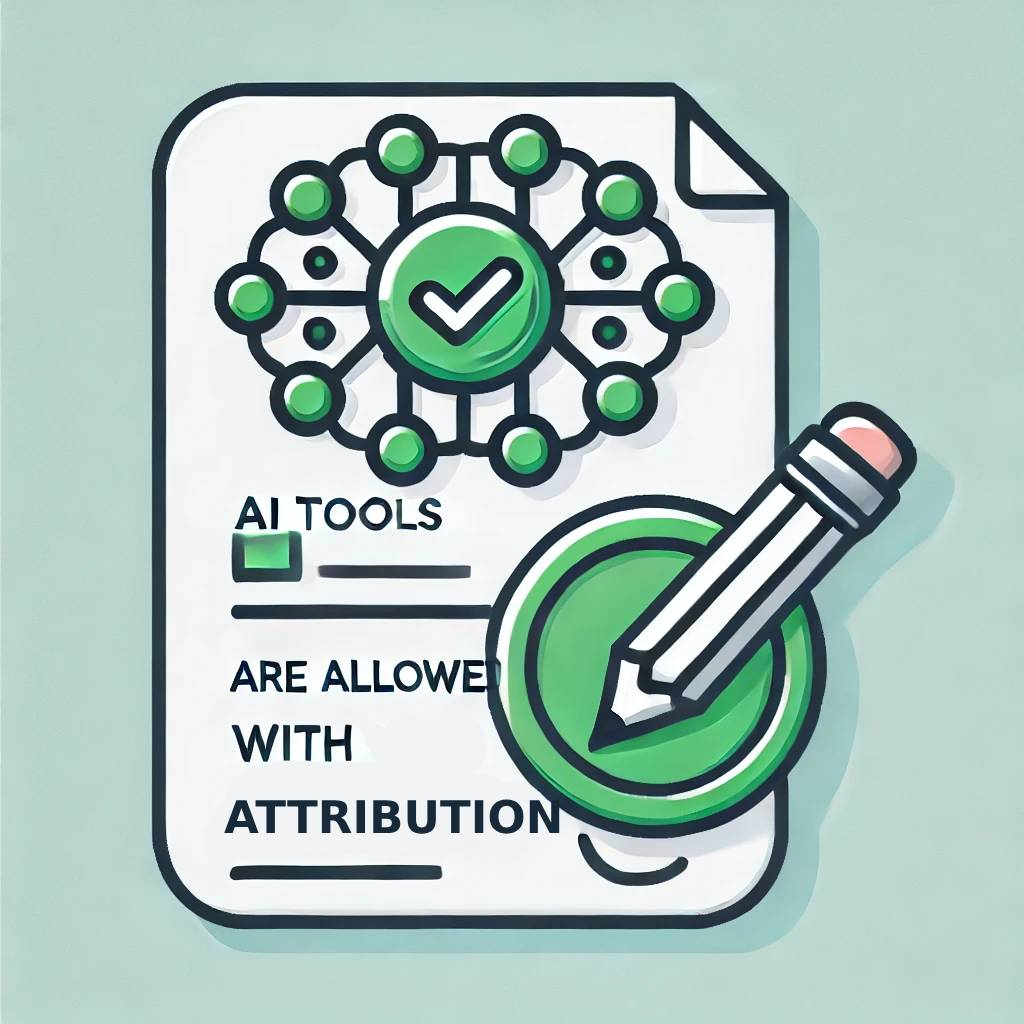
\includegraphics[width=1cm]{figs/Allowed_with_contributino.jpg}
    در این تمرین با مدل \lr{ViT} برای دسته‌بندی تصاویر آشنا خواهید شد. شما یک مدل \lr{pretrained}  را با استفاده از \lr{Hugging Face} بارگذاری می‌کنید، وزن‌های \lr{attention} آن را تجزیه و تحلیل می‌کنید و برای درک بهتر مکانیزم توجه و رفتار آن در مدل پیش آموخته شده، وزن‌های یادگیری شده را نمایش خواهید داد. در بخش بعدی آن را روی دیتاست \lr{CIFAR-10}  آموزش خواهید داد ( \lr{fine-tune}) و در نهایت نقش \lr{attention head}ها را بررسی می‌کنید. در این سوال از نوتبوک \lr{Q5.ipynb} استفاده کنید.(۲۵ نمره)
    \begin{enumerate}
        \item از کتابخانه \lr{transformers} در \lr{Hugging Face} برای بارگذاری مدل \lr{pretrained} استفاده کنید (ترجیحا مدل \lr{google/vit-base-patch16-224}). در این بخش پس از انجام پیش‌پردازش تصویر مورد نظر، با استفاده از مدل پیش‌آموزش دیده خروجی مدل را بدست آورده و ۵ کلاس برتر پیش‌بینی شده را  همراه با احتمالات پیش‌بینی محاسبه کنید. 
        \item با فراخوانی مدل می‌توانید به وزن‌های مکانیزم توجه برای تصویر مورد‌نظر دسترسی داشته باشید. در این بخش \lr{attention weights} مربوط به توکن [\lr{CLS}] را استخراج کنید و نقشه‌های توجه این توکن را برای تمام لایه و \lr{head}ها به صورت جداگانه نمایش دهید.
        \item \href{https://aclanthology.org/2020.acl-main.385.pdf}{\lr{Attention Rollout}} روشی برای مصورسازی و تفسیر مکانیزم توجه در مدل‌های \lr{Transformer} است. در این روش با ضرب تجمعی ماتریس‌های \lr{attention} در لایه‌ها، مسیر توجه از ورودی تا خروجی مدل به‌صورت یکپارچه نمایش داده می‌شود. با استفاده از روش \lr{attention rollout} و توضیحات داخل نوتبوک جریان تاثیر هر \lr{patch} از تصویر روی توکن \lr{cls} را در طول لایه‌ها نمایش دهید. 
        \item مدل پیش‌آموخته شده را بر روی دیتاست \lr{CIFAR-10} آموزش (\lr{fine-tune}) دهید و دقت آن را گزارش کنید. 
        \item در این بخش پس از آموزش روی دادگان بررسی کنید که دور ریختن یک یا چند \lr{head} چه تاثیری در عملکرد مدل ایجاد می‌کند. با استفاده از داده \lr{validation} تحلیل کنید کدام \lr{head}ها نقش مهمتری در تصمیم‌گیری مدل دارند.  
    \end{enumerate}
    \textcolor{blue}{\textbf{برای استفاده از پاسخنامه به پوشه \lr{Q5-HW4-solution} مراجعه کنید که از پاسخ آقای پولایی استفاده شده است.}}
    \item 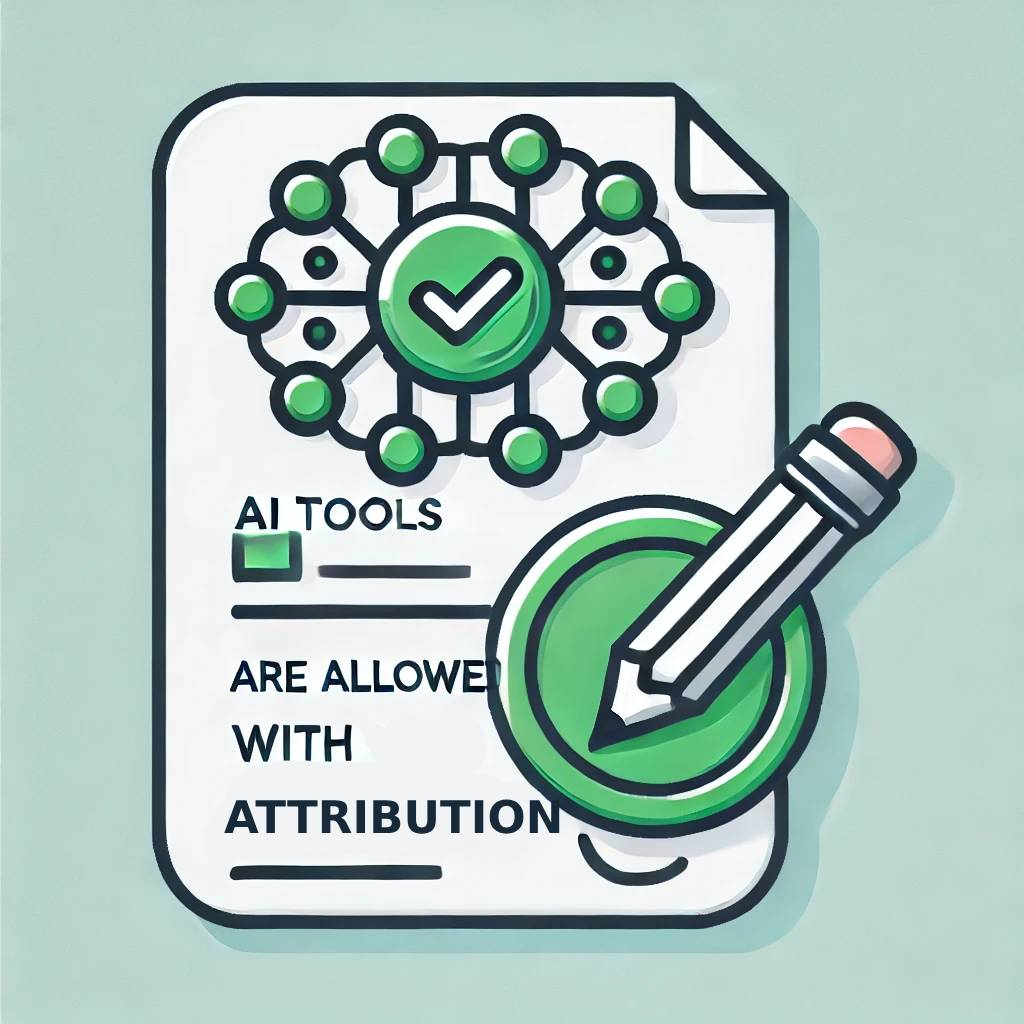
\includegraphics[width=1cm]{figs/Allowed_with_contributino.jpg}
    در این تمرین، مدل ترجمه ماشینی مبتنی بر توجهی را آموزش خواهید داد تا کلمات را از انگلیسی به \lr{Pig-Latin}    ترجمه کنید.\lr{Pig-Latin}یک بازی زبانی است که در آن قوانین به صورت مستقل برای هر کلمه اعمال می    شود:    (۲۵ نمره)
    \begin{itemize}
        \item اگر اولین حرف یک کلمه، حرف بی صدای انگلیسی باشد، آن حرف به انتهای کلمه منتقل شده و حروف \lr{\lr{ay}}به انتهای کلمه اضافه می  شوند: \lr{team → eamtay} .
        \item  اگر اولین حرف، یک حرف صدادار انگلیسی باشد، کلمه بدون تغییر باقی می ماند و حروف \lr{way } به انتهای کلمه اضافه می شوند: \lr{impress → impressway}.
        \item برخی از جفت حروف مانند \lr{sh} به عنوان یک بلوک در نظر گرفته  میشوند و به صورت کل به انتهای رشته منتقل میشوند:
        \lr{shopping → oppingshay}
    \end{itemize}
    هدف این است که مدل ترجمه ماشینی قوانین را به طور ضمنی از طریق جفت های کلمات (\lr{English}, \lr{Pig-Latin}) که \lr{source}  کلمه انگلیسی و \lr{target} ترجمه آن به  \lr{Pig-Latin} است، یاد بگیرد.\\
    داده ها:\\
    در این تمرین از دو مجموعه داده استفاده خواهید کرد:\\
    \begin{itemize}
    \item واژگان مجموعه داده کوچک شامل ۲۹ نشانه است: ۲۶ حرف استاندارد الفبا (همه با حروف کوچک)، نماد خط تیره “-” و دو نشانه \lr{<SOS>} و \lr{<EOS>} که به ترتیب شروع و پایان یک دنباله را نشان می‌دهند. مجموعه داده شامل ۳۱۹۸ جفت (\lr{English}, \lr{Pig-Latin}) منحصر به فرد است.
    \item مجموعه داده بزرگ‌تر، شامل 2۰,۰۰۰ کلمه انگلیسی پرکاربردتر است که با مجموعه داده قبلی ترکیب می‌شود و 22402 کلمه منحصر به فرد به دست می‌آید
    \end{itemize}
    \begin{enumerate}
    \item به بخش \lr{scaled dot product attention} در نوتبوک \lr{pigLatin} مراجعه کرده و بخش‌های مشخص‌شده را تکمیل کنید.
    \item مدل \lr{Transformer} را با استفاده از \lr{hidden size}  های 32 و 64 و با استفاده از مجموعه داده کوچک و بزرگ (در مجموع ۴ اجرا) اجرا کنید و اثرات افزایش ظرفیت مدل از طریق \lr{hidden size} و افزایش اندازه مجموعه داده را گزارش کنید.
    \item به معماری \lr{Transformer} در شکل زیر نگاه کنید. در هر لایه ابتدا \lr{CausalScaledDotAttention} را به ورودی‌های \lr{decoder} و سپس \lr{ScaledDotAttention} را به \lr{encoder annotations} اعمال می‌کنیم. \lr{\_\_init\_\_} بخش \lr{decoder} را طوری تغییر دهید که فقط از \lr{ScaledDotAttention} استفاده کند. نتایج خود را حالت قبلی مقایسه کنید.
    \end{enumerate}
    \begin{figure}[h]  
            \centering
            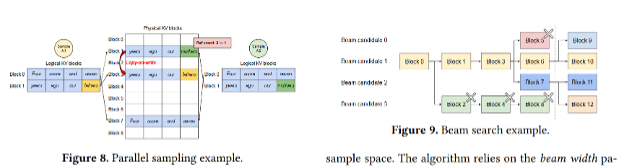
\includegraphics[width=\textwidth]{figs/Q1_3.png}
            \label{fig:num_pic}  
        \end{figure}
    \textcolor{blue}{\textbf{برای استفاده از پاسخنامه به پوشه \lr{Q6-HW4-solution} مراجعه کنید که از پاسخ آقای حسین زاده استفاده شده است.}}

\end{enumerate}



\end{document}


